%!TEX root = ../main.tex

We show how to use \cosette for debugging JavaScript code annotated with 
separation logic (SL) specifications. Tools that allow for SL-reasoning about
functional correctness properties in general, and those targeting 
JavaScript in particular, require of the user to have substantial expertise 
and to go through a long and complex proof trace in order to find the precise 
source of an error. \cosette substantially simplifies this process by providing
concrete counter-models that invalidate the specification.
In \S\ref{subsec:sep:assertions}, we extend the 
 \jsil symbolic interpreter with a mechanism for asserting
SL-assertions. 
In \S\ref{subsec:countermodels}, we show how to implement this mechanism by giving a sound decision procedure for finding counter-models 
for SL-assertions.
In \S\ref{specs:to:symbolic:tests}, we present an algorithm  
for generating symbolic tests from SL-specifications, which guarantees 
that if a symbolic test fails, then Cosette must produce a concrete 
counter-model that invalidates 
the specification. Finally, in~\S\ref{specs:example}, we show how to use the 
proposed methodology for debugging JaVerT specifications~\cite{javert} of JavaScript~code. 

\subsection{\jsil Symbolic Execution with Separation Logic Assertions}
\label{subsec:sep:assertions}

We extend \jsil with a special construct, $\sepassert(P)$, for stating that 
the separation logic assertion $P$ must hold whenever $\sepassert(P)$ is evaluated. 
We use the assertion language of~\cite{javert}, with the following adaptation:
instead of \emph{untyped logical variables}, we 
use \emph{typed logical variables}, $\svar \in \svars$, which include 
symbolic numbers, $\snumber \in \snumbers$, strings $\sstring \in \sstrings$, 
and locations,~$\sloc \in \slocs$. 

\myparagraph{\jsil assertions: syntax and semantics}
\jsil assertions include: boolean operations; first-order connectives; the separating conjunction; 
existential quantification; and assertions for describing heaps. The $\lemp$ assertion describes 
an empty heap. The cell assertion, $(\lexpr_1,\lexpr_2) \pointsto \lexpr_3$,  describes an object 
at the location denoted by $\lexpr_1$ with a property denoted by $\lexpr_2$ that has the value 
denoted by $\lexpr_3$. The assertion $\emptyfields{\lexpr_1}{\lexpr_2}$ states that the object at 
the location denoted by $\lexpr_1$ has no properties other than possibly those included in the
set denoted by $\lexpr_2$. 
%
As in~\cite{gardner:popl:2012,javert}, in order to define the semantics of assertions, 
we resort to \emph{instrumented heaps} $\iheap \in \iheaps$, which differ from 
concrete heaps in that they may map object properties to the special value $\none$, 
explicitly indicating that the property does not exist (e.g. $\iheap(\loc, \jstring) = \none$
means that the object at location $\loc$ in the heap $\iheap$ does not have a property
named~$\jstring$). 
%Analogously, we extend symbolic heaps with $\none$-cells, obtained \emph{instrumented symbolic heaps} $\isheap \in \isheaps$. 
Instrumented heaps are related to heaps by means of an \emph{erasure 
function}, $\deabstract{.}: \iheaps \rightarrow \heaps$, %($\deabstract{.}: \isheaps \rightarrow \sheaps$), 
which simply removes the none-cells from the instrumented heap given as input.  Below, we give the syntax and semantics of \jsil assertions. Note that we assume pure assertions to have an empty spatial footprint and allow logical negation, conjunction, and disjunction of pure formulae only.

%  \deabstract{\jsilaheap}(\loc, x) = \jsilaheap(\loc, x) \iffdef (\loc, x) \in \domain(\jsilaheap) \ \wedge \ \jsilaheap(\loc, x) \neq \none

\begin{display}{\jsil Logic Assertions - Syntax and Semantics}
%
{\scriptsize \begin{tabular}{lll}
  %%%% 
  $\quad \lexpr \triangleq$ & $\lit \mid \jvar \mid \svar \mid \unoper\ \lexpr \mid \lexpr \binoper \lexpr$ &   \text{ Logical Expressions} \\[3pt]
  %%%%
  $\quad P_\pc\triangleq$ & $\jtrue \mid \jfalse \mid  \neg P_\pc \mid P_\pc \land P_\pc \mid P_\pc \lor P_\pc  \mid \lexpr = \lexpr \mid \lexpr \leq \lexpr$ & \text{~{Pure Assertions}} \\
  $\quad P\triangleq$ & $P_\pc \mid \lemp \mid (\lexpr, \lexpr)\pointsto \lexpr \mid \exists \svar. P \mid P \sep P  \mid \emptyfields{\lexpr}{\lexpr} $ &  \text{~Assertions} \\
\end{tabular}} \\ [5pt]
  %%%%%
  %%%%%
  
\quad 
{\scriptsize
\begin{tabular}{lll} 
       $\iheap, \store, \senv  \satisfies  \lemp$ & $\Leftrightarrow$ & $\iheap = \hemp$  \\[2pt]
           %
	   $\iheap, \store, \senv  \satisfies (\lexpr_1,\lexpr_2)\pointsto \lexpr_3$  &
            $\Leftrightarrow$ & $\iheap =  \hcell{\symbeval{\lexpr_1}{\store, \senv}}{\symbeval{\lexpr_2}{\store, \senv}}{\symbeval{\lexpr_3}{\store, \senv}}$  \\[2pt]
           % 
           $\iheap, \store, \senv  \satisfies P \sep Q$ & $\Leftrightarrow$ & $\exists \iheap_1, \iheap_2.  \, \iheap = \iheap_1 \dunion \iheap_2\ \wedge \ \iheap_1,  \store, \senv  \satisfies P \, \wedge \, \iheap_2,  \store, \senv \satisfies Q$ \\[2pt]
           %
           $\iheap, \store, \senv  \satisfies  \emptyfields{\lexpr_1}{\lexpr_2}$  &
                $\Leftrightarrow$ & $\iheap = \biguplus_{s \not\in \{ \symbeval{\lexpr_2}{\store, \senv} \}} ((\symbeval{\lexpr_1}{\store, \senv}, s) \pointsto \none)$
\end{tabular}}
\end{display}
%
For convenience, we define: 
\begin{align}
\sepmodels{P} = \left\{ (\heap, \store, \senv) \mid \exists \iheap \, . \,  \heap = \deabstract{\iheap} \ \wedge \ \iheap, \store, \senv \satisfies P  \right\}
\end{align}
Given a symbolic heap $\sheap$, a symbolic store $\sstore$, a path condition $\pc$, and 
an assertion $P$, we say that  $(\sheap, \sstore, \pc)$ \emph{satisfies} $P$, 
written $\sheap, \sstore, \pc \satisfies P$ \emph{if and only if}
$\smodels{\sheap, \sstore}{\pc} \subseteq \sepmodels{P}$. 
%
We can now give an \emph{ideal} symbolic semantics for the command $\sepassert(P)$ (which checks
if the current symbolic state satisfies $P$): 

\polish{the configurations need to be updated with the bot or top in the appropriate place. It appears 3 times: below, 
when the rules are re-stated with a call to the decision procedure, in Theorem 8.}
{\small \begin{mathpar}
\inferrule[\textsc{Assert - True}]
  { 
     \sheap, \sstore, \pc \satisfies P
  }{\symbtrans{\sheap, \sstore, \sepassert(P), \pc}{\sheap, \sstore, \pc}} 
\and
\inferrule[\textsc{Assert - False}]
  { 
          \sheap, \sstore, \pc \not\satisfies P
  }{\symbtranserr{\sheap, \sstore, \sepassert(P), \pc}{}{\pc}} 
\end{mathpar}}
\hspace{-3pt}Determining whether or not a symbolic state satisfies an SL-assertion $P$ is, in general, 
undecidable \cite{citemeplease}. Since we do not want to produce \emph{false positives}, in order to trigger 
an assertion failure, we need to find a concrete witness for that failure. More precisely, when executing 
$\sepassert(P)$ in the symbolic state $(\sheap, \sstore, \pc)$, the symbolic analysis must  
report an assertion failure only if it can find a concrete state $(\heap, \store)$  and a symbolic environment 
$\senv$ such that: 
$(\heap, \store, \senv) \in \smodels{\sheap, \sstore}{\pc}$ and
$(\heap, \store, \senv) \not\in \sepmodels{P}$.

%\begin{figure}[t!]
%\centering
%{\scriptsize
%\begin{mathpar} 
%\inferrule[\textsc{New Existential}]
%     { 
%         \svar \in \existentials 
%         \quad
%         \svar \not\in \domain(\subst)
%     }
%     {\unification{\sexpr, \pc}{\svar}{\subst}{\existentials} = \uyes{\subst[\svar \mapsto \sexpr]}}
%\quad
%\inferrule[\textsc{Matched Existential}]
%     { 
%         \subst(\svar) = \sexpr' 
%         \quad 
%         \pc \vdash \sexpr = \sexpr' 
%     }
%     {\unification{\sexpr, \pc}{\svar}{\subst}{\existentials} = \uyes{\subst}}
%\quad
%\inferrule[\textsc{Existential - None}]
%     { 
%         \subst(\svar) = \sexpr' 
%         \quad 
%         \pc \not\vdash \sexpr = \sexpr' 
%     }
%     {\unification{\sexpr, \pc}{\svar}{\subst}{\existentials} = \uno{\sexpr \neq \sexpr'}}
%\\
%\inferrule[\textsc{Grounded Expression}]
%     { 
%         \fv(\subst(\sexpr')) \cap \existentials = \emptyset
%         \quad 
%          \pc \vdash  \sexpr = \subst(\sexpr') 
%     }
%     {\unification{\sexpr, \pc}{\sexpr'}{\subst}{\existentials} = \uyes{\subst}}
%\qquad
%\inferrule[\textsc{Grounded Expression - Fail}]
%     { 
%         \fv(\subst(\sexpr')) \cap \existentials = \emptyset
%         \quad 
%          \pc  \not\vdash  \sexpr = \subst(\sexpr') 
%     }
%     {\unification{\sexpr, \pc}{\sexpr'}{\subst}{\existentials} = \uno{\sexpr  \neq \subst(\sexpr')}}
%%
%\\
%%
%\\
%\inferrule[\textsc{None-Cell Assertion}]
%	{  
%	   \subst(\symbeval{\lexpr_l}{\sstore})  = \loc 
%	   \quad 
%	    \symbeval{\lexpr_p}{\sstore} = \sexprp' 
%	   \quad
%       \sheap = \sheap' \dunion  \big((l, \sexprp_i) \mapsto \sexprv_i\big)\mid_{i = 0}^n    
%	   \quad
%	   (l, -) \not\in \domain(\sheap')  
%	   \quad
%	    \pc \vdash \sexprp' \not\in \{ \sexprp_i \mid_{i = 0}^n \} 
%	}{ \unification{\sheap, \sstore, \pc}{(\lexpr_l,\lexpr_p)\pointsto \none}{\subst}{\existentials} = \uyes{\subst, \sheap}} 
%%
%\\
%\inferrule[\textsc{None-Cell Assertion - Fail}]
%	{  
%	   \subst(\symbeval{\lexpr_l}{\sstore})  = \loc 
%	   \quad 
%	    \symbeval{\lexpr_p}{\sstore} = \sexprp' 
%	   \quad
%       \sheap = \sheap' \dunion  \big((l, \sexprp_i) \mapsto \sexprv_i\big)\mid_{i = 0}^n    
%	   \quad
%	   (l, -) \not\in \domain(\sheap')  
%	   \quad
%	    \pc \not\vdash \sexprp' \not\in \{ \sexprp_i \mid_{i = 0}^n \} 
%	}{ \unification{\sheap, \sstore, \pc}{(\lexpr_l,\lexpr_p)\pointsto \none}{\subst}{\existentials} = \uno{\sexprp' \in \{ \sexprp_i \mid_{i = 0}^n \} }} 
%%
%\\
%\inferrule[\textsc{EmptyFields Assertion}]
%	{  
%	  \loc = \subst(\symbeval{\lexpr_l}{\sstore}) 
%	   \quad 
%	     \symbeval{\lexpr_d}{\sstore} = \sexprv' 
%	   \quad
%	     \sheap = \sheap' \, \uplus \, \big((l, \sexprp_i) \mapsto \sexprv_i\big)\mid_{i = 0}^n   
%              \quad
%             (l, -) \not\in \domain(\sheap')
%	    \quad 
%	    \pc \vdash \big( \{ \sexprp_i \mid_{i = 0}^n   \} \subseteq \sexprv' \big)
%	}{ \unification{\sheap, \sstore, \pc}{\emptyfields{\lexpr_l}{\lexpr_d}}{\subst}{\existentials} = \uyes{(\subst, \sheap)}} 
%\\
%\inferrule[\textsc{EmptyFields Assertion - Fail}]
%	{  
%	   \loc = \subst(\symbeval{\lexpr_l}{\sstore}) 
%	   \quad 
%	     \symbeval{\lexpr_d}{\sstore} = \sexprv' 
%	   \quad
%	     \sheap = \sheap' \, \uplus \, \big((l, \sexprp_i) \mapsto \sexprv_i\big)\mid_{i = 0}^n   
%              \quad
%             (l, -) \not\in \domain(\sheap')
%	    \quad 
%	    \pc \not\vdash \big( \{ \sexprp_i \mid_{i = 0}^n   \} \subseteq \sexprv' \big)
%	}{ \unification{\sheap, \sstore, \pc}{\emptyfields{\lexpr_l}{\lexpr_d}}{\subst}{\existentials} = \uno{\{ \sexprp_i \mid_{i = 0}^n   \} \not\subseteq \sexprv'}} 
%\end{mathpar}
%\hrule
%\caption{Unification of spatial assertions:
% {\scriptsize$\unification{\sheap, \sstore, \pc}{\cell}{\subst}{\existentials} = \uyes{\subst', \sheap_f} \texttt{ OR } \uno{\pc'}$}}\label{fig:unification}}
%\end{figure}


\begin{table}
\centering
\renewcommand{\arraystretch}{1.2} 
{\scriptsize \begin{tabular}{@{}cccccccc@{}}\toprule
\multicolumn{3}{c}{{\it Symbolic State}} & &  & & & \\
\cmidrule{1-3}% \cmidrule{4-4}
\emph{Heap}  &  & \emph{PC}  &   &  \emph{Assertion}  & & \emph{Failing Constraint}       \\
\cmidrule{1-1} \cmidrule{3-3} \cmidrule{5-5}  \cmidrule{7-7}
%
$(\loc, \sexprp_1) \mapsto \sexprv$ & & $\jtrue$ & & 
	$(\loc, \sexprp_2) \mapsto \sexprv$ & &  $\sexprp_1 \neq \sexprp_2$ \\    
%
$(\loc, \sexprp_1) \mapsto \sexprv$ & & $\jtrue$ & & 
	$(\loc, \sexprp_1) \mapsto \sexprv \sep (\loc, \sexprp_2) \mapsto \none$ & &  $\sexprp_1 = \sexprp_2$ \\    
%
$(\loc, \sexprp_1) \mapsto \sexprv$ & & $\sexprp_1 \neq \sexprp_2$ & & 
	$(\loc, \sexprp_1) \mapsto \sexprv \sep (\loc, \sexprp_2) \mapsto \none \sep \emptyfields{\loc}{\{\sexprp_2, \sexprp_3\}}$ & &  $\sexprp_1 \neq \sexprp_3$ \\    
%
$(\loc, \sexprp_1) \mapsto \sexprv$ & & $\sexprp_1 \not\in \{\sexprp_2, \sexprp_3\}$ & & 
	$(\loc, \sexprp_1) \mapsto \sexprv \sep (\loc, \sexprp_2) \mapsto \none \sep (\loc, \sexprp_3) \mapsto \none$ & &  $\sexprp_2 = \sexprp_3$ \\    

\bottomrule
\end{tabular}}
\vspace{2pt}
\caption{Symbolic States vs Assertions\label{example:symb:states:vs:assertions}}
\vspace*{-0.7cm}
\end{table}

\subsection{Finding Counter Models for SL Assertions}
\label{subsec:countermodels}

We describe a partial decision procedure, which we  
implement as part of the \jsil symbolic interpreter, for proving entailments 
between symbolic states and SL-assertions \underline{and} finding counter 
models in case of failure.  
% I have to give more examples
As it is customary~\cite{javert,jacobs2011verifast,sepwithsmt}, the decision procedure works by first using \emph{pattern-matching} 
on the spatial part of the SL-assertion, and then discharging the pure part of the 
entailment to an external constraint solver (in our case, \rosette). 

\myparagraph{Representation of SL-assertions}
We target SL-assertions $P$ that can be represented as quadruples,
$(\existentials, \cells, \efs, \pfs)$, consisting of: 
\dtag{1} a set $\existentials$ of existentially quantified symbolic locations, 
\dtag{2} a list $\cells$ containing the non-none cell assertions (those whose value is different from $\none$), 
\dtag{3} a set $\efs$ containing the none-cell assertions and the empty-fields assertions, and
\dtag{4} a pure assertion $\pfs$. 
Hence, letting $\existentials = \{ \sloc_1, ..., \sloc_k \}$, $\cells = [ \cell_i \mid_{i = 0}^n ]$, and
$\efs = \{\efa_i \mid_{i = 0}^m \}$, we write $P \equiv (\existentials, \cells, \efs, \pfs)$ as shorthand for: 
 \begin{equation}
P = \exists \sloc_1, ..., \sloc_k \, . \big( \bigoast_{0 \leq i \leq n} \cell_i \ \sep  \bigoast_{0 \leq i \leq m} \efa_i \big) \ \lstar \ \pfs
\end{equation}
Given a symbolic state $(\sheap, \sstore, \pc)$ and an assertion $P \equiv (\existentials, \cells, \efs, \pfs)$, 
we represent each possible mapping from the existentially quantified symbolic locations in $P$ 
to the concrete locations in $\sheap$ as a \emph{substitution function} $\subst : \slocs \rightharpoonup \locs$.
Since both $\existentials$ and the set of concrete locations in $\sheap$ 
are finite, we conclude that there is a finite number of substitution functions to be considered 
when checking if $(\sheap, \sstore, \pc)$ satisfies $P$. 
Hence, in the following, we will assume a fixed substitution,~$\subst$. %\polish{Does this paragraph need to be rewritten? Stores?}
Furthermore, we assume that the SL-assertion given as input to the decision procedure does not contain any program variables. This we justify by noting that the following equivalence holds (the proof can be found in the Appendix):  
\begin{equation}
 \sheap, \sstore, \pc \satisfies P \iff \sheap, \emptystore, \pc \satisfies \symbeval{P}{\sstore},
\end{equation}
where $\symbeval{P}{\sstore}$ denotes the SL-assertion obtained by symbolically evaluating 
all the symbolic expressions in $P$ under $\sstore$.
%To obtain an SL-assertion in the targeted format, it suffices to symbolically evaluate all its symbolic expressions under the appropriate symbolic store. 



\begin{figure}[!t]
{\scriptsize
\begin{mathpar} 
\inferrule[\textsc{Cell Assertion}]
	{  
	    \sheap = \sheap_f \dunion ((l, \sexprp') \mapsto \sexprv') 
	   \\\\
	    \pc \vdash  \sexprp = \sexprp' \wedge \sexprv = \sexprv'
	}{\cellunification{\sheap, ((\loc,\sexprp)\pointsto \sexprv) \lstcons \cells}{\sheap_f, \cells}{\pc}} 
\and
\inferrule[\textsc{Cell Assertion - Fail}]
	{  
	   \sheap = \sheap' \dunion  \big((l, \sexprp_i) \mapsto \sexprv_i\big)\mid_{i = 0}^n  
	   \quad 
	     l \notin \hlocs{\sheap'}
	    \\\\ 
	     \pc_i = (\sexprp_i = \sexprp' \wedge \sexprv_i = \sexprv')\!\mid_{i = 0}^n
	    \quad
	    \pc \not\vdash \pc_i \mid_{i = 0}^n
	}{  \cellunificationx{\sheap, ((\loc,\sexprp)\pointsto \sexprv) \lstcons \cells}{\uno{\wedge_{0 \leq i \leq n} \neg\pc_i}}\pc } 
\end{mathpar}}
\vspace*{-0.5cm}
\caption{Unification of non-none cells: $\cellunification{\sheap, \cells}{\sheap_f, \cells'}{\pc}$
and $\cellunificationx{\sheap, \cells}{\uno{\pc'}}{\pc}$}
%$\unification{\sheap, \pc}{\cell}{} = \uyes{\sheap_f} \texttt{ or } \uno{\pc'}$}
\label{fig:uninonnone}
\vspace*{-0.2cm}
\end{figure}


\myparagraph{Unification rules}
In Figure \ref{fig:uninonnone}, we show the unification rules for non-none cell assertions. 
We write $\cellunificationx{\sheap, \cell \lstcons \cells}{-}\pc$ to denote the unification of a symbolic heap $\sheap$ against a single non-none cell $\cell$, given a path condition $\pc$.\footnote{We denote the transitive closure of $\rightarrow_{\mathcal{CU}}$ by $\rightarrow_{\mathcal{CU}}^*$.}  This unification can either terminate
successfully, with $\tuple{\sheap_f, \cells}$, in which case $\sheap_f$ denotes the
symbolic heap %to be framed off
that \underline{does not} contain the footprint of $\cell$, 
 and $\cells$ denotes the list of remaining non-none cell assertions to be unified (\textsc{Cell Assertion}); or unsuccessfully, with $\uno{\pc'}$, 
in which case $\pc'$ captures the constraints required for the unification to provably fail (\textsc{Cell Assertion - Fail}).
For instance, in the first example of Table~\ref{example:symb:states:vs:assertions}, 
in order to generate a witness for the entailment failure, we need to instantiate $\sexprp_1$ and $\sexprp_2$ so that the \emph{failing constraint} $\sexprp_1 \neq \sexprp_2$ is satisfied. 

%Given a cell assertion $\cell$, a symbolic state $(\sheap, \pc)$, 
%and a substitution $\subst$: 
%\begin{itemize}
%    \item if $\unification{\sheap, \pc}{\cell}{} = \uyes{\sheap_f}$, then there are 
%            two heaps $\sheap'$ and $\sheap_f$, such that $\sheap = \sheap' \dunion \sheap_f$
%            and $\smodels{\sheap', -}{\pc} \subseteq \sepmodels{\cell}$; 
%   
%   \item if $\unification{\sheap, \pc}{\cell}{} = \uno{\pc'}$, then there are 
%            no two heaps $\sheap'$ and $\sheap_f$, such that $\sheap = \sheap' \dunion \sheap_f$ 
%            and $\smodels{\sheap', -}{\pc \, \wedge \, \pc'} \subseteq \sepmodels{\cell}$.
%\end{itemize}

%\vspace{-3pt}
%\begin{display}{Unification of negative-resource assertions: $\unificationef{\sheap}{\efs} = \pc$ and $\sanity{\efs} = \pc$}

Unification of negative resource, that is, none-cells and \jsinline|emptyFields| assertions, is more intricate, as symbolic heaps do not maintain negative information. We denote by $\unificationef{\sheap}{\efs}$ the constraints that need to be satisfied for the unification of a symbolic heap $\sheap$ against the negative resource denoted by $\efs$ to succeed, and show the rules in Figure \ref{fig:unineg}. First, unifying a symbolic heap $\sheap$ that contains the object $\loc$ with properties $\sexprp_i|_{i=0}^n$ against a none-cell $(\loc,\sexprp)\pointsto \none$ effectively means that $\sexprp$ has to be different from all $\sexprp_i|_{i=0}^n$ (\textsc{NR-None Cell}). Next, unifying a symbolic heap $\sheap$ that contains the object $\loc$ with properties $\sexprp_i|_{i=0}^n$ against an  \jsinline|emptyFields| assertion $\emptyfields{\loc}{\sexpr_d}$ means that all of the properties $\sexprp_i|_{i=0}^n$  have to be in the domain of of the \jsinline|emptyFields| assertion, $\sexpr_d$ (\textsc{NR-Empty Fields}). 
The second and third examples of Table~\ref{example:symb:states:vs:assertions} illustrate unification failures resulting from NR-constraints not being satisfied: the second example targets the (\textsc{NR-None Cell}) rule, with the failing constraint: $\sexprp_1 \neq \sexprp_2$; and the third example targets the (\textsc{NR-Empty Fields}) rule, with the failing constraint $\sexprp_1 \not\in \jsilset{\sexprp_2, \sexprp_3}$.

\begin{figure}[!t]
{\scriptsize
\begin{mathpar} 
\inferrule[\textsc{NR-None Cell}]
	{  
	   \sheap = \sheap' \, \uplus \, \big((l, \sexprp_i) \mapsto -\big)\mid_{i = 0}^n   
	   \\\\
	    l \notin \hlocs{\sheap'}
	    \quad 
	    \pc = \wedge_{0 \leq i \leq n} \sexprp \neq \sexprp_i 
	 }{ \unificationefl{\sheap}{(\loc,\sexprp)\pointsto \none} =  \pc  }
\qquad
\inferrule[\textsc{NR-Empty Fields}]
	{  
	    \sheap = \sheap' \dunion  \big((l, \sexprp_i) \mapsto -\big)\mid_{i = 0}^n   
	    \\\\
	     l \notin \hlocs{\sheap'}
	     \quad 
	    \pc = \{ \sexprp_i \mid_{i = 0}^n \} \subseteq \sexpr_d 
	}{ \unificationefl{\sheap}{\emptyfields{\loc}{\sexpr_d}}{} =  \pc  } 
%
\\

\inferrule[\textsc{NR-Unification}]
	{}{ \unificationef{\sheap}{\efs} =  \bigwedge_{\efa \in \efs}  \unificationefl{\sheap}{\efa}} 
\\
\inferrule[\textsc{Separation Constraints - Fixed Location}]
	{
		 \efproj{\efs}{\loc} = \emptyfields{\loc}{\sexpr_d} \sep  \oast_{i = 0}^{n} \, \big((l, \sexprp_i) \mapsto \none \big)
	}{ \sanityl{\efs}{\loc} = 
		 (\wedge_{0 \leq i, j \leq n, i \neq j} \sexprp_i \neq \sexprp_j)
		       \, \wedge \,  ( \wedge_{0 \leq i \leq n} \sexprp_i \in \sexpr_d )
	} 
\and
\inferrule[\textsc{Separation Constraints}]
	{}{ \sanity{\efs} = \bigwedge_{\loc \in \eflocs(\efs)}\sanityl{\efs}{\loc}} 
\end{mathpar}}
\vspace*{-0.6cm}
\caption{Unification of negative-resource assertions: $\unificationef{\sheap}{\efs} = \pc$ and $\sanity{\efs} = \pc$}
\label{fig:unineg}
\vspace*{-0.2cm}
\end{figure}

Furthermore, due to the semantics of the separating conjunction, there are additional  constraints imposed by the negative resource. Concretely, all none-cells for the same object have to have different property names, and if any none-cell is starred together with an \jsinline|emptyFields| assertion for the same object, then its property name has to be in the domain of that \jsinline|emptyFields| assertion (\textsc{Separation-Constraints - Fixed Location}). 
We call these constrants \emph{separation constraints}, and denote them, for a fixed location~$\loc$, by $\sanityl{\efs}{\loc}$ in Figure~\ref{fig:unineg}. The point is that, if a given symbolic state entails a negative resource assertion, it must be the case that its path condition entails the corresponding separation constraints.
The last example of Table~\ref{example:symb:states:vs:assertions} illustrates a unification failure resulting from an EF-separation-constraint not being satisfied,
namely $\sexprp_2 \neq \sexprp_3$. 

Finally, the (\textsc{NR-Unification}) and (\textsc{Separation Constraints}) rules extend $\unificationef{\sheap}{\efs}$ and $\sanityl{\efs}{\loc}$, respectively, to sets of negative resource formulas.

\begin{figure}[t!]
{\scriptsize
\centering
\begin{mathpar} 
\inferrule[\textsc{Fail - Cell Unification}]
	{  
	   \cellunificationiterx{\sheap, \cells}{\uno{\pc''}}{\pc}
	}{\unificationfullfail{\sheap, \pc}{\cells, \efs, \pfs'}{}{\pc''}} 
\and
\inferrule[\textsc{Fail - Extra Resource}]
	{  
	     \cellunificationiter{\sheap, \cells}{\sheap_f, []}{\pc}
	     \qquad
	     \sheap_f \neq \hemp
	}{\unificationfullfail{\sheap, \pc}{\emptyset, \efs, \pfs'}{}{\jtrue}} 
\\
%
%
\inferrule[\textsc{Fail - Pure Entailment}]
	{  
	   \cellunificationiter{\sheap, \cells}{\hemp, []}{\pc}
	   \\\\
	   \pc'' = \unificationef{\sheap}{\efs} \wedge \, \sanity{\efs}
	   \quad
             \pc \not\vdash \pfs' \, \wedge \, \pc''
	}{\unificationfullfail{\sheap, \pc}{\cells, \efs, \pfs'}{}{\neg(\pc'  \, \wedge \, \pc'')}} 
\and
\inferrule[\textsc{Success}]
	{     
	   \cellunificationiter{\sheap, \cells}{\hemp, []}{\pc}
	   \\\\
	   \pc \vdash \pfs' \, \wedge \, \unificationef{\sheap}{\efs}   \, \wedge \, \sanity{\efs}
	}{\unificationfull{\sheap, \pc}{\cells, \efs, \pfs'}{}} 
%
\end{mathpar}}
\vspace*{-0.6cm}
\caption{Unification algorithm: {\small $\unificationfull{\sheap, \pc}{\cells, \efs, \pfs'}{}$}
and {\small $\unificationfullfail{\sheap, \pc}{\cells, \efs, \pfs'}{}{\pc'}$}.\label{unification:algorithm}}
\vspace*{-0.3cm}
\end{figure}

%\pmax{Stopped here.}

\myparagraph{Unification Algorithm}
Figure~\ref{unification:algorithm} presents the rules for the \emph{unification algorithm}. 
We write $\unificationfull{\sheap, \pc}{\cells, \efs \pfs'}{}$ to mean that the unification of 
the symbolic state $\sheap, \pc$ against the assertion $P \equiv (\emptyset, \cells, \efs, \pfs')$ 
succeeds, and $\unificationfullfail{\sheap, \pc}{\cells, \efs, \pfs'}{}{\pc'}$ to mean that it
fails, with the \emph{failing constraints} being: $\pc'$. Note that in order to generate a 
witness for the unification failure, one needs to find a symbolic environment satisfying the 
failing constraints.

The algorithm works by trying to unify the non-none cell assertions first. 
The unification succeeds when they are all successfully unified, the resulting symbolic heap is empty, 
and the final pure entailment is discharged by the constraint solver (\textsc{Success}). 
On the other hand, the unification can fail in three
ways: 
a non-none cell may not be unifiable (\textsc{Fail - Cell Unification}); 
all non-none cells are unifiable, but there may be additional resource left (\textsc{Fail - Extra Resource}); 
and all non-none cells are unifiable, there is no additional resource left, but the final
pure entailment may not be discharged by the constraint solver (\textsc{Fail - Pure Entailment}). 
Note that in case of failure, the algorithm 
always returns the constraints that need to be satisfied for a witness of that failure to be produced. 

Below we present the rules of the unification algorithm for a general assertion $P$.
For clarity, we use $\substs(\existentials, \sheap)$ to denote the set of all substitutions
mapping symbolic location in $\existentials$ to concrete locations in the domain of $\sheap$. 
%
For the success case, we simply need to find a substitution $\subst$ 
for which the unification algorithm terminates successfully. For the failure case, 
we need to compute the failing constraints for all possible substitutions, and 
return their conjunction. 


\begin{display}{Unification of General Assertions}
\inferrule[\textsc{Success}]
 { 
    \exists \subst . \, \symbeval{\subst(P)}{\sstore} \equiv (\emptyset, \cells, \efs, \pfs')
    \\\\ \unificationfull{\sheap, \pc}{\cells, \efs, \pfs'}{}
 }{\unificationfullP{\sheap, \sstore, \pc}{P}{}}
%
 \qquad
 %
 \inferrule[\textsc{Failure}]
 { 
     P \equiv (\existentials, -, -, -) 
     %
     \qquad
     %
     \substs(\existentials, \sheap) = \{ \subst_1, ..., \subst_n \}
    \\\\
     \forall_{1 \leq k \leq n}  . \, \big( \symbeval{\subst(P)}{\sstore} \equiv (\emptyset, \cells, \efs, \pfs') 
           \, \wedge \,  \unificationfullfail{\sheap, \pc}{\cells, \efs, \pfs'}{}{\pc_k}  \big)
     %
 }{\unificationfullfailP{\sheap, \sstore, \pc}{P}{\wedge_{0 \leq k \leq n} \pc_k}}
 \end{display}

We can now give the \emph{implemented} symbolic semantics for the command $\sepassert(P)$ 
which makes use of the unification algorithm described above: 
{\small \begin{mathpar}
\inferrule[\textsc{Assert - True}]
  { 
      \unificationfullP{\sheap, \sstore, \pc}{P}{}
  }{\symbtrans{\sheap, \sstore, \sepassert(P), \pc}{\sheap, \sstore, \pc}} 
\and
\inferrule[\textsc{Assert - False}]
  {  
       \unificationfullfailP{\sheap, \sstore, \pc}{P}{\pc'}  
      \qquad
      (\pc \, \wedge \, \pc') \text{ is satisfiable}  
  }{\symbtranserr{\sheap, \sstore, \sepassert(P), \pc}{}{\pc \, \wedge \, \pc'}} 
\end{mathpar}}


\myparagraph{Soundness}
Theorem \ref{teo:unification:soundness} states that the unification algorithm is sound: given an SL-assertion~$P$ and a 
symbolic state $(\sheap, \sstore, \pc)$, if $\unificationfullP{\sheap, \sstore, \pc}{P}{}$ then the symbolic state
$(\sheap, \sstore, \pc)$ satisfies~$P$. 
The bug-finding theorem, Theorem \ref{teo:bugfinding}, is more subtle. It states that, in case of failure,  to find a counter-model 
for $P$, one has to pick a concretisation of the symbolic state that is consistent with 
the failing constraint generated by the unification algorithm. 



\begin{theorem}[Soundness of Unification]\label{teo:unification:soundness}
$\forall P, \sheap, \sstore, \pc \, .$
$$
\begin{array}{l}
   \unificationfullP{\sheap, \sstore, \pc}{P}{}
    \implies \smodels{\sheap, \sstore}{\pc} \subseteq \sepmodels{P}   
\end{array}
$$ 
\end{theorem}


\begin{theorem}[Bug-finding for SL]\label{teo:bugfinding}
$\forall P, \sheap, \sstore, \pc.$
$$
\unificationfullfailP{\sheap, \sstore, \pc}{P}{\pc'} \implies 
   \smodels{\sheap, \sstore}{\pc \wedge \pc'} \cap \sepmodels{P} = \emptyset
$$ 
\end{theorem}
%
The {\bf proofs} of the above results are given in the Appendix.

%\begin{theorem}[Soundness of Unification]\label{teo:unification:soundness}
%$\forall P, \cells, \efs, \pfs',  \sheap, \sstore, \pc, \subst \, .$
%$$
%\begin{array}{l}
%\symbeval{\subst(P)}{\sstore} \equiv (\emptyset, \cells, \efs, \pfs')\implies\unificationfull{\sheap, \pc}{\cells, \efs, \pfs'}{} \
%    \implies \smodels{\sheap, \sstore}{\pc} \subseteq \sepmodels{P}   
%\end{array}
%$$ 
%\end{theorem}
%
%
%\begin{theorem}[Bug-finding for SL]\label{teo:bugfinding}
%$\forall P, \existentials, \sheap, \sstore, \pc, \pc'.$
%$$
%\begin{array}{l}
%   P \equiv (\existentials, -, -, -) \implies \\
%   \quad \big( \forall \subst, \cells, \efs, \pfs''.\ \subst \in \substs(\existentials, \sheap) \implies 
%   \symbeval{\subst(P)}{\sstore} \equiv (\emptyset, \cells, \efs, \pfs'') \implies \\
%   \qquad \unificationfullfail{\sheap, \pc}{\cells, \efs, \pfs''}{}{\pc'''} \ \wedge \  \pc' \vdash \pfs''' \big) \implies \\
%   \qquad \quad \smodels{\sheap, \sstore}{\pc \wedge \pc'} \cap \sepmodels{P} = \emptyset.   
%\end{array}
%$$ 
%\end{theorem}



\subsection{Compiling \jsil Logic Specifications to Symbolic Tests}
\label{specs:to:symbolic:tests}

\begin{figure*}
\begin{center}
$$
\begin{array}{ll}
\testify{\fnormal}(\fid, \svar_i\mid_{i=0}^n, \pc, Q) \ \semeq & \\
         \dspc \dspc  \darkmath{\sf proc} \jsilmain () \{ 
         &  \text{Generated testing procedure for \underline{normal}-return specification:} \\ 
             \dspc \dspc \dspc 0_{\phantom{\sf nm}}:  \assume(\pc) 
                   & \text{  {\bf a.} Assume the initial path condition} \\ 
   %
             \dspc \dspc \dspc 1_{\phantom{\sf nm}}: \jsilcall{\jvar}{\fid}{\svar_0, ..., \svar_n}{\procerrlab}  
                   & \text{  {\bf b.} Call the procedure to be tested $\fid$ with symbolic arguments $\svar_i\mid_{i=0}^n$} \\ 
             \dspc \dspc \dspc \procretlab \, : \sepassert(Q[\jvar/\procretvar])
                  & \text{  {\bf c.}  In case of normal return, assert the $\fnormal$-postcondition of $\fid$} \\ 
             \dspc \dspc \dspc \procerrlab \, \, \, : \assert(\jfalse)
                  & \text{  {\bf d.}  In case of error return, assert $\jfalse$} \\ 
         \ \ \ \ \ \ \ \} &\\[8pt]
%
\testify{\ferror}(\fid, \svar_i\mid_{i=0}^n, \pc, Q) \ \semeq & \\
         \dspc \dspc  \darkmath{\sf proc} \jsilmain () \{ 
         &  \text{Generated testing procedure for \underline{error}-return specification:} \\ 
            \dspc \dspc \dspc 0_{\phantom{\sf nm}}:  \assume(\pc)   
                   & \text{  {\bf a.} Assume the initial path condition} \\ 
             \dspc \dspc \dspc 1_{\phantom{\sf nm}}: \jsilcall{\jvar}{\fid}{\svar_0, ..., \svar_n}{\procerrlab}  
                   & \text{  {\bf b.} Call the procedure to be tested $\fid$ with symbolic arguments $\svar_i\mid_{i=0}^n$} \\ 
             \dspc \dspc \dspc \procretlab \, : \assert(\jfalse)
                  & \text{  {\bf c.}  In case of normal return, assert $\jfalse$} \\ 
             \dspc \dspc \dspc \procerrlab \, \, \, : \sepassert(Q[\jvar/\procerrvar])
                  & \text{  {\bf d.}  In case of error return,  assert the $\ferror$-postcondition of $\fid$} \\ 
         \ \ \ \ \ \ \ \} \\[8pt]
%         
\testify{}(\specsig{P}{\fid(\jvec{x})}{Q}{\flag}) \ \semeq & \\      
    \dspc \dspc  \mathbf{let} \ \subst = \mathbf{pick} \ \functionset{\aslocs(P)}{\locs \backslash \eflocs(P)} \ \mathbf{in} 
           & \text{  {\bf a.}  Compute a substitution from the symbolic locations in $P$ to} \\ 
           & \text{ $\phantom{a.}\ $ randomly picked concrete locations not overlapping with those in $P$}  \\
    %
    \dspc \dspc  \mathbf{let} \ (-, \cells, \efs, \pc) = \subst(P) \ \mathbf{in}  
            & \text{  {\bf b.}  Apply the substitution to $P$ obtaining $(-, \cells, \efs, \pc)$}  \\
    %
    \dspc \dspc  \mathbf{let} \ \sstore = [ \jvar_i \mapsto \svar_i \mid_{i=0}^n] \ \mathbf{in} 
            & \text{  {\bf c.} Compute the initial store mapping each argument to a symbolic}  \\
            & \text{ $\phantom{c.} \ $  value of the appropriate type}  \\
       %
    \dspc \dspc  \mathbf{let} \ \sheap = \symbeval{\cells}{\sstore} \ \mathbf{in} 
           & \text{  {\bf d.}  Symbolically evaluate $\efs$ under $\sstore$, obtaining $\sheap$}  \\
     %
    \dspc \dspc  \mathbf{let} \ \pc' = \sanity{\symbeval{\efs}{\sstore}} \, \wedge \,  \unificationef{\sheap}{\symbeval{\efs}{\sstore}}  \ \mathbf{in} 
           & \text{  {\bf e.}  Compute the appropriate NR- and separation constraints}  \\
    %
      \dspc \dspc  \mathbf{let} \ \pc'' = \symbeval{\subst(\pc)}{\sstore} \, \wedge \, \pc'  \ \mathbf{in} 
          & \text{  {\bf f.} Construct the initial path condition from $\pc$ and $\pc'$}  \\
    %
       \dspc \dspc  \mathbf{let} \ \proc = \testify{\flag}(\fid, \svar_i\mid_{i=0}^n, \pc'', \symbeval{\subst(Q)}{\sstore})  \ \mathbf{in} 
          & \text{  {\bf g.} Synthesise the symbolic test} \\
     %
      \dspc \dspc \dspc (\proc, \sheap) 
\end{array}
$$
\vspace*{-0.2cm}
\caption{Symbolic Test Generation Algorithm~\label{fig:test:generation}}
\vspace*{-0.2cm}
\end{center}
\end{figure*}


\myparagraph{\jsil Logic specifications}
\jsil Logic specifications have the form $\specsig{P}{\fid(\jvec{x})}{Q}{\flag}$, where $P$ and $Q$ are the 
pre- and postconditions of the function with identifier $\fid$, and $\jvec{x}$ its list of formal parameters.
Each specification is associated with a return mode $\flag \in \{ \fnormal, \ferror \}$, indicating if the function
 returns normally or with an error. If it returns normally, then its return value can be accessed  via a dedicated variable 
 $\procretvar$, and $\procerrvar$ otherwise.  Intuitively, a specification $\specsig{P}{\fid(\jvec{x})}{Q}{\flag}$ is 
valid for a given \jsil program $\prog$, if $\prog$ contains a procedure with identifier 
$\fid$ and ``whenever $\fid$ is executed in a state satisfying $P$, then, 
if it terminates, it does so in a state satisfying $Q$, with return mode $\flag$''.
The formal definition is given below. 


\begin{definition}[Validity of \jsil Logic Specifications]
A \jsil logic specification $\specsig{P}{\fid(\jvec{x})}{Q}{\flag}$ is valid with respect to a program 
$\prog$, written $\prog \satisfies \specsig{P}{\fid(\jvec{x})}{Q}{\flag}$,  if and only if, for all logical 
contexts $(\iheap, \store, \senv)$, heaps $\heap_f$, stores $\store_f$, and flags $\flag'$, it holds that: 
$$
\begin{array}{l}
    \iheap, \store, \senv \satisfies P \ \wedge \ \tuple{\deabstract{\iheap}, \store, \ctx[0]} \rightarrow^* \tuple{\heap_f, \store_f, \ctx[i_{\flag'}]} \\
       \quad \implies
            \flag' = \flag \ \wedge \ \exists \iheap_f \, . \, \iheap_f, \store_f, \senv \satisfies Q \ \wedge \ \deabstract{\iheap_f} = \heap_f
\end{array}
$$
\end{definition}

\myparagraph{Symbolic test generation}
\noindent Given a \jsil program $\prog$ containing a procedure $\fid$ with spec {\small $\specsig{P}{\fid(\jvec{x})}{Q}{\flag}$}, 
our goal is to construct a symbolic test for checking whether or not $\fid$ behaves as its specification mandates.
A symbolic test is a pair $(\proc, \sheap)$ consisting of a \jsil procedure with the code of the test and the initial 
symbolic heap on which to execute the test. 
%
Figure~\ref{fig:test:generation} presents the test generation procedure. Intuitively, $\testify{}(\specsig{P}{\fid(\jvec{x})}{Q}{\flag})$ 
returns the symbolic test for $\specsig{P}{\fid(\jvec{x})}{Q}{\flag}$. The test generation function $\testifyfun{}$ is defined in terms 
of two auxiliary functions, $\testifyfun{\fnormal}$ and $\testifyfun{\ferror}$, for generating tests for $\fnormal$-mode and 
$\ferror$-mode specifications, respectively. 
The test program $\prog'$, denoted by $\prog[\jsilmain \mapsto \proc]$, is obtained from the original program $\prog$ and the test procedure $\proc$ by replacing the 
$\jsilmain$ of $\prog$ with the new test procedure, $\proc$. 
%
Finally, Theorem~\ref{teo:bug:finding:sl} states that if the symbolic execution of the 
test generated for $\specsig{P}{\fid(\jvec{x})}{Q}{\flag}$ finds a bug, then the specification 
is not~valid.

\begin{theorem}[Bug-finding for SL Specifications]\label{teo:bug:finding:sl}
$$
\begin{array}{l}
\testify{}(\specsig{P}{\fid(\jvec{x})}{Q}{\flag})  = (\proc, \sheap) \, \wedge \, 
   \prog[\jsilmain \mapsto \proc] : \symbtranstranserr{\sheap, [], i, \pc}{\sctxmain}{\pc'} \\
  \qquad \qquad \implies
        \prog \not\satisfies \specsig{P}{\fid(\jvec{x})}{Q}{\flag}
\end{array}
$$
\noindent where $\sctxmain$ denotes the initial call stack: $[ (\jsilmain, -, -, -) ]$.
\end{theorem}


\myparagraph{Symbolic States versus SL-Assertions} 
Note that the conversion of the 
precondition $P$ of a \jsil procedure $\fid$ to a symbolic state $(\sheap, \sstore, \pc)$ involves transforming the negative resource assertions in $P$ into pure constraints encoded by the initial path condition $\pc$ and not captured by $\sheap$.
We will illustrate this with an example in the following section. 

\myparagraph{Inductive Predicates} 
\cosette does not have built-in abstraction mechanisms. Hence, it does not support symbolic
execution over inductive predicates describing recursive data structures, which are 
commonplace in separation-logic-style specifications~\cite{smallf, berdine:aplas:2005}. 
As in~\cite{korat}, we deal with user-defined inductive predicate assertions by \emph{unfolding} 
those assertions up to a fixed bound, which is established by the user. This unfolding mechanism 
is routine
%\footnote{Ooooooooooooooooooooooooooooooooooooooooo...} 
and its details are, therefore, omitted from the paper. 


\subsection{Compiling JaVerT Specifications to Symbolic Tests} 
\label{specs:example}

\myparagraph{\javert Specifications} 
\javert specifications of JavaScript functions are analogous to \jsil specifications of \jsil procedures, and are of the form $\specsig{P_{\jssuffix}}{\fid(\jvec{x})}{Q_{\jssuffix}}{\flag}$. A~\javert specification $\specsig{P_{\jssuffix}}{\fid(\jvec{x})}{Q_{\jssuffix}}{\flag}$
is valid for a JavaScript program $\jstmt$, written $\jstmt \satisfies \specsig{P_{\jssuffix}}{\fid(\jvec{x})}{Q_{\jssuffix}}{\flag}$, 
if and only if $\jstmt$ contains a function literal with identifier $\fid$ and ``whenever $\fid$ is executed in a state satisfying $P_\jssuffix$, then, 
if it terminates, it does so in a state satisfying $Q_\jssuffix$, with return mode $\flag$''. The assertion language used by \javert is very similar to the assertion language of \jsil Logic and is described in detail in~\cite{javert}.
There, the authors present 
a compiler from \javert specifications to \jsil Logic specifications, denoted by $\ltr$, and prove the soundness 
of that compiler, assuming a correct compiler $\compile$ from JavaScript to~\jsil.
This theoretical result ensures that the verification of \jsil programs can be lifted to   the verification of JavaScript programs. More concretely, a \javert  specification $\specsig{P_{\jssuffix}}{\fid(\jvec{x})}{Q_{\jssuffix}}{\flag}$
is valid for a given JavaScript program $\jstmt$ if and only if the translated specification 
$\ltr(\specsig{P_{\jssuffix}}{\fid(\jvec{x})}{Q_{\jssuffix}}{\flag})$ is valid for the compilation 
of $\jstmt$ by a correct compiler $\compile$. Put formally:  
\begin{equation}
   \jstmt \vDash  \specsig{P_{\jssuffix}}{\fid(\jvec{x})}{Q_{\jssuffix}}{\flag} 
      \iff
           \compile(\jstmt) \vDash \ltr(\specsig{P_{\jssuffix}}{\fid(\jvec{x})}{Q_{\jssuffix}}{\flag}).
\end{equation}

We generate symbolic tests from JavaScript programs and their \javert specifications in the following way. First, we convert the JavaScript program and its \javert specification to a \jsil program with its \jsil Logic specification, using the \JSComp and $\ltr$ compilers. Next, we 
generate a set of symbolic tests from the obtained \jsil program and \jsil Logic specification, as described in \S\ref{specs:to:symbolic:tests}. 
Finally, we run the generated \jsil symbolic tests on the \jsil symbolic execution engine. If \cosette finds a bug while running these tests, we will obtain a concrete counter-example triggering that bug.

\begin{figure}[t!]
\centering
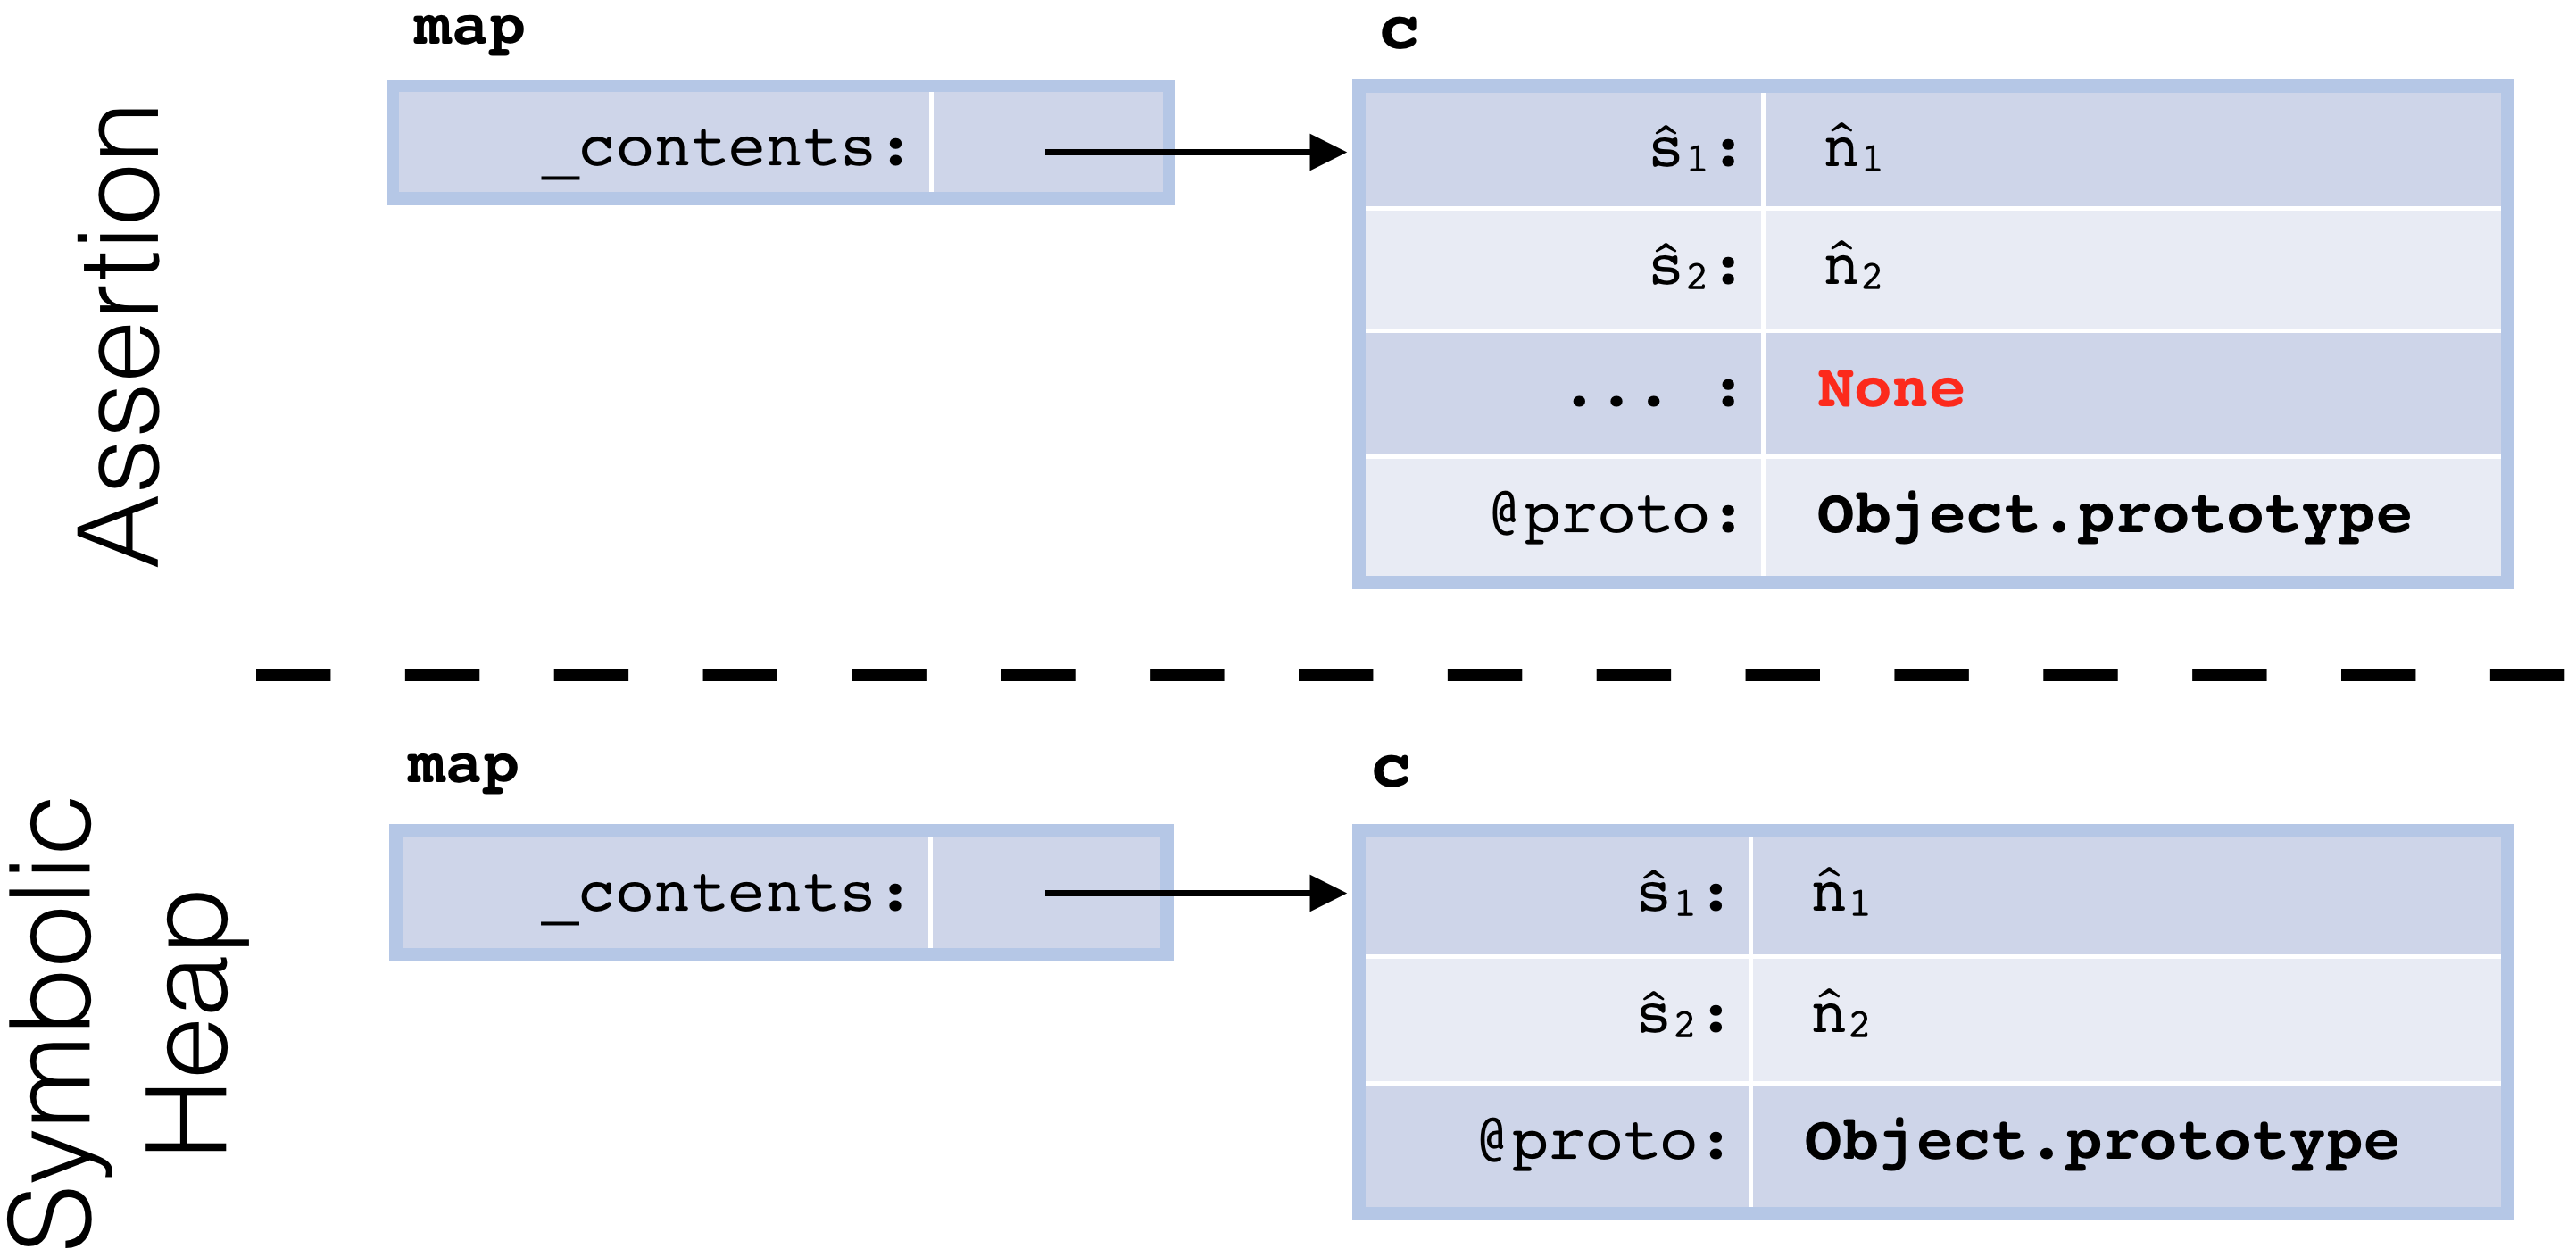
\includegraphics[width=\linewidth]{figures/symbvsass.png}

\vspace*{-0.7cm}
{\small $$
\text{\emph{Negative resource constraints: }} \{ \hat{s}_1, \hat{s}_2 \} \subseteq \{ \hat{s}_1, \hat{s}_2 \}
$$}
\vspace{-0.8cm}
\caption{Assertion vs. Symbolic Heap: {\small$\mathtt{Map(map, \{ (\hat{s}_1, \hat{n}_1), (\hat{s}_2, \hat{n}_2) \} )}$}}\label{fig:symb:state:versus:assertion}
\vspace{-0.5cm}
\end{figure}

\myparagraph{Example}
We illustrate the debugging of SL-specifications by appealing to the \jsinline|Map| example shown in Figure \ref{map:example}. In order to reason about a key-value map,
we define several predicates, whose definitions we show below.

\begin{Verbatim}[fontsize=\footnotesize,commandchars=\\\{\}]
Map (m, kvs) := 
  DataProp(m, "_contents", c) * JSObject(c) * 
    KVPairs(c, kvs) * first(kvs, keys) * emptyFields(c, keys)
\end{Verbatim}
 \begin{Verbatim}[fontsize=\footnotesize,commandchars=\\\{\}]
KVPairs (o, kvs) := 
  (kvs = \{ \}),
  (kvs = (k, v) -u- kvs') * ValidKey(k) * DataProp(o, k, v) * KVPairs(o, kvs')
\end{Verbatim}
\begin{Verbatim}[fontsize=\footnotesize,commandchars=\\\{\}]
ValidKey (k) := types(k : Str) * \textcolor{red}{(k <> "hasOwnProperty")}
\end{Verbatim}

The \jsinline|Map| predicate captures the resource corresponding to a map object. 
Concretely, it first states that the map object has the property \jsinline|_contents|, which points to a default JavaScript object \jsinline|c|, using the predicates \jsinline|DataProp| and \jsinline|JSObject|. 
\jsinline|DataProp(o, p, v)| captures the property \jsinline|p| of object \jsinline|o| and states that it has value \jsinline|v|, while abstracting over other associated JavaScript internals, whereas \jsinline|JSObject(o)| states that the object \jsinline|o| is an extensible object of class \jsinline|"Object"|, whose prototype is \jsinline|Object.prototype| (for more details, see~\cite{javert}). 
Next, using the \jsinline|KVPairs| predicate (explained shortly), it states that \jsinline|c| holds the key-value pairs \jsinline|kvs|. Finally, it states that \jsinline|c| has no other properties except the keys present in \jsinline|kvs|. For this, it first obtains the set of keys from the set of key-value pairs \jsinline|kvs| using the predicate \jsinline|first(kvs, keys)|, which states that the first projection of \jsinline|kvs| equals \jsinline|keys| (its definition is standard), and then uses the \jsinline|emptyFields| assertion to state that all other properties are absent from the object.

The \jsinline|KVPairs(o, kvs)| predicate talks about key-value pairs of an object \jsinline|o|. 
It is defined recursively on the structure of \jsinline|kvs| and it has two definitions, separated by a comma. 
We have that \jsinline|kvs| is either empty or that it contains at least one key-value pair \jsinline|(k, v)|.\footnote{We write {\small\texttt{-u-}} for set union and omit the brackets around singleton sets.} 
In the latter case, we state that the key \jsinline|k| must be valid, that the object \jsinline|o| has the property \jsinline|k| with value \jsinline|v|, and proceed recursively.
Note that the uniqueness of keys in \jsinline|kvs| is guaranteed by the \jsinline|DataProp| predicate of \jsinline|KVPairs| and the separating conjunction.

The \jsinline|ValidKey(k)| predicate captures the validity of a given key and holds \emph{iff} the corresponding JavaScript function \jsinline|validKey(k)| returns \jsinline|true|.
In the definition of \jsinline|ValidKey|, we highlight in red a potential source of errors on which we will focus shortly.

To give a better intuition of how the \jsinline|Map| predicate works, we show the full unfolding of {\small$\mathtt{Map(map, \{ (\hat{s}_1, \hat{n}_1), (\hat{s}_2, \hat{n}_2) \} )}$} in Figure \ref{fig:symb:state:versus:assertion}.
%a \emph{map object predicate}, \jsinline|Map|, 
%which uses the auxiliary predicate \jsinline|KVPairs|, capturing the resource of the key-value pairs in the map, 
%and the \jsinline|validKey(k)| predicate, which captures the validity of a key and holds if and only if the corresponding JavaScript function \jsinline|ValidKey(k)| returns \jsinline|true|\footnote{For the moment, we treat the $\mathtt{ValidKey}$ predicate as a black box.}.
%
%Intuitively, the \jsinline|Map(m, kvs)| predicate captures the resource 
%of a map object \jsinline|m| with key-value pairs \jsinline|kvs| (a set of string-number pairs, modelled as two-element lists).
%%\footnote{We model pairs as lists with two elements and, for clarity, use the pair notation.}). 
%For instance, the assertion $\mathtt{Map(map, \{ (\hat{s}_1, \hat{n}_1), (\hat{s}_2, \hat{n}_2) \} )}$ can be unfolded as illustrated in Figure~\ref{fig:symb:state:versus:assertion}. 
%Observe that the definition of \jsinline|Map| does not include the resource of a map prototype, as it is shared between all map objects, and therefore needs to be factored out.  
%
There, we can also see how the negative resource captured by the SL-assertion {\small$\mathtt{Map(map, \{ (\hat{s}_1, \hat{n}_1), (\hat{s}_2, \hat{n}_2) \} )}$}, namely the resource captured by {\small$\mathtt{emptyFields(c, first(kvs))}$}, disappears from the symbolic heap and is transformed into the negative resource constraint $\{ \hat{s}_1, \hat{s}_2 \} \subseteq \{ \hat{s}_1, \hat{s}_2 \}$, which states that all properties of the object \jsinline|c| in the symbolic heap (in our case, $\hat{s}_1$ and $\hat{s}_2$) must be in the set of properties of the corresponding \jsinline|emptyFields| assertion (in our case, {\small$\mathtt{first(\{ (\hat{s}_1, \hat{n}_1), (\hat{s}_2, \hat{n}_2) \}) = \{ \hat{s}_1, \hat{s}_2 \}}$}).
Such constraints are generated in item ${\bf e.}$ of the test generation algorithm presented in Figure \ref{fig:test:generation}. 

Below, we show the relevant parts of the specifications of \jsinline|get(k)| and \jsinline|put(k, v)|, for the case in which
 \jsinline|k| already exists in the map:

\noindent
\begin{minipage}{\linewidth}
\begin{displaymath} 
{\scriptsize
\hspace*{-0.2cm}
\begin{array}{c}
\left\{ {\begin{array}{c}
 \text{\texttt{Map(this, kvs -u- (k, v)) * ObjProtoF() *}} \\
 \text{\texttt{(this, "@proto") -> mp * MapProto(mp) * ...}}
\end{array}} \right\} \\
%
\text{\bfseries \texttt{get(k)}} \\[0.2mm]
%
\left\{ {\begin{array}{c}
 \text{\texttt{Precondition * (ret = v)}} 
\end{array}} \right\}
\end{array}
} 
\end{displaymath}
\end{minipage}
\quad
\begin{minipage}{\linewidth}
%
\begin{displaymath} 
{\scriptsize
\begin{array}{c}
\left\{ {\begin{array}{c}
 \text{\texttt{Map(this, kvs -u- (k, v')) * ObjProtoF() *}} \\
 \text{\texttt{(this, "@proto") -> mp * MapProto(mp) * ...}}
\end{array}} \right\} \\
%
\text{\bfseries \texttt{put(k, v)}} \\[0.2mm]
%
\left\{ {\begin{array}{c}
 \text{\texttt{Map(this, kvs -u- (k, v)) * ObjProtoF() *}} \\
 \text{\texttt{(this, "@proto") -> mp * MapProto(mp) * ...}}
\end{array}} \right\}
\end{array}
} 
\end{displaymath}
\end{minipage}

\vspace{10pt}
The predicate \jsinline|ObjProtoF()| describes the resource captured by the \jsinline|Object.prototype| object. 
In particular, it is needed because \texttt{get} uses the \texttt{hasOwnProperty} function, which is defined as a property of \jsinline|Object.prototype|. 
The predicate \jsinline|MapProto| specifies the resource of a valid map prototype: in particular, the map prototype needs to define the methods \jsinline|put|, \jsinline|get|, and \jsinline|validKey|. Finally, note that, given the definition of the \jsinline|Map| and \jsinline|KVPairs| predicates, both preconditions shown entail that \jsinline|k| is a valid key.

\begin{figure}[t!]
\centering
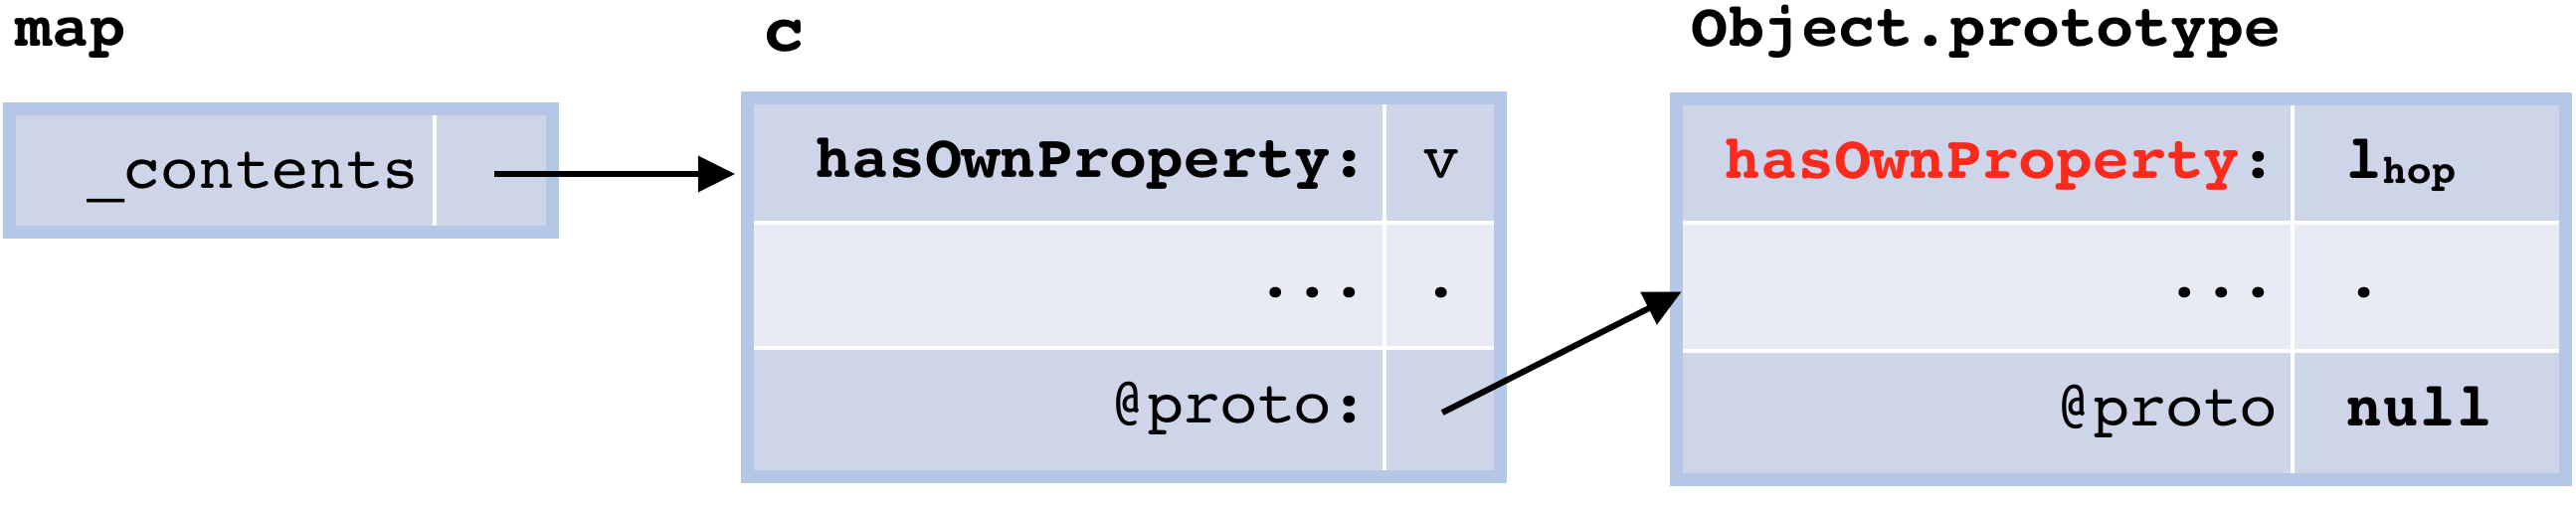
\includegraphics[width=\linewidth]{figures/heapfail.png}
\caption{Property shadowing: \jsinline|c.hasOwnProperty(...)| cannot reach \jsinline|Object.prototype|.} 
\label{fig:cexget}
\vspace{-0.5cm}
\end{figure}

Now, if we forgot to state the part of the $\mathtt{ValidKey(k)}$ predicate highlighted in red, that is, if we did not state that $\mathtt{k}$ needed to be different from \jsinline|"hasOwnProperty"|, the symbolic test generated for the specification of \jsinline|get| would fail for unfoldings of $\mathtt{KVPairs}$ of depth $\geq 1$, with the counter-model \jsinline|k = "hasOwnProperty"|. 
In that case, as illustrated in Figure~\ref{fig:cexget}, the \jsinline|"hasOwnProperty"| property of \jsinline|Object.prototype| would no longer be reachable by property lookup from \jsinline|c|, and
the execution of line~5 (\jsinline|if (c.hasOwnProperty(k))|) would raise an error, as it would attempt to call the \jsinline|"hasOwnProperty"| property of object \jsinline|c| as a function instead. 
Since this specification of $\mathtt{get(k)}$ requires normal termination, the jump to the error label in the compiled \jsil code will trigger the $\assert(\jfalse)$ of the generated symbolic test and the developer will be presented with the counter-model \jsinline|k = "hasOwnProperty"|.

\begin{center}
\polish{What else would we like to say here?}
\end{center}

%%
%% OLD THINGS

%\begin{figure}[t!]
%\centering
%{\scriptsize
%\begin{mathpar} 
%\inferrule[\textsc{New Existential}]
%     { 
%         \svar \in \existentials 
%         \quad
%         \svar \not\in \domain(\subst)
%     }
%     {\unification{\sexpr, \pc}{\svar}{\subst}{\existentials} = \optionsome{\subst[\svar \mapsto \sexpr]}}
%\quad
%\inferrule[\textsc{Matched Existential}]
%     { 
%         \subst(\svar) = \sexpr' 
%         \quad 
%         \pc \vdash \sexpr = \sexpr' 
%     }
%     {\unification{\sexpr, \pc}{\svar}{\subst}{\existentials} = \optionsome{\subst}}
%\quad
%\inferrule[\textsc{Existential - None}]
%     { 
%         \subst(\svar) = \sexpr' 
%         \quad 
%         \pc \vdash \sexpr \neq \sexpr' 
%     }
%     {\unificationfail{\sexpr, \pc}{\svar}{\subst}{\existentials} = \optionnone}
%\\
%\inferrule[\textsc{Grounded Expression}]
%     { 
%         \fv(\subst(\sexpr')) \cap \existentials = \emptyset
%         \quad 
%          \pc \vdash  \sexpr = \subst(\sexpr') 
%     }
%     {\unification{\sexpr, \pc}{\sexpr'}{\subst}{\existentials} = \optionsome{\subst}}
%\qquad
%\inferrule[\textsc{Grounded Expression - Fail}]
%     { 
%         \fv(\subst(\sexpr')) \cap \existentials = \emptyset
%         \quad 
%          \pc  \vdash  \sexpr \neq \subst(\sexpr') 
%     }
%     {\unification{\sexpr, \pc}{\sexpr'}{\subst}{\existentials} = \optionnone}
%%
%\\
%\inferrule[\textsc{Cell Assertion}]
%	{  
%	   \big(\loc = \symbeval{\lexpr_l}{\sstore} \ \vee \loc = \subst(\symbeval{\lexpr_l}{\sstore}) \big)
%	   \quad 
%	     \symbeval{\lexpr_p}{\sstore} = \sexprp'
%	   \quad
%	   \symbeval{\lexpr_v}{\sstore} = \sexprv' 
%	   \quad
%	    \sheap = \sheap_f \dunion ((l, \sexprp) \mapsto \sexprv) 
%	   \\
%	   \unification{\sexprp, \pc}{\sexprp'}{\subst}{\existentials} = \optionsome{\subst'} 
%	   \quad
%	   \unification{\sexprv, \pc}{\sexprv'}{\subst'}{\existentials} = \optionsome{\subst''} 
%	}{ \unification{\sheap, \sstore, \pc}{(\lexpr_l,\lexpr_p)\pointsto \lexpr_v}{\subst}{\existentials} = \optionsome{(\subst'', \sheap_f)}} 
%\\
%\inferrule[\textsc{Cell Assertion - Fail}]
%	{  
%	   \big(\loc = \symbeval{\lexpr_l}{\sstore} \ \vee \loc = \subst(\symbeval{\lexpr_l}{\sstore}) \big)
%	   \quad
%	     \symbeval{\lexpr_p}{\sstore} = \sexprp'
%	   \quad
%	   \symbeval{\lexpr_v}{\sstore} = \sexprv' 
%	   \quad
%	     \sheap = \sheap' \dunion  \big((l, \sexprp_i) \mapsto \sexprv_i\big)\mid_{i = 0}^n   
%  	   \\
%	    (l, -) \not\in \domain(\sheap') 
%	    \quad 
%	   \forall_{0 \leq i \leq n} \, \unification{\sexprp, \pc}{\sexprp'}{\subst}{\existentials} = \optionnone 
%	   \ \vee \
%	   \unification{\sexprv, \pc}{\sexprv'}{\subst'}{\existentials} = \optionnone
%	}{ \unification{\sheap, \sstore, \pc}{(\lexpr_l,\lexpr_p)\pointsto \lexpr_v}{\subst}{\existentials} = \optionnone} 
%\\
%\inferrule[\textsc{EmptyFields Assertion}]
%	{  
%	   \big(\loc = \symbeval{\lexpr_l}{\sstore} \ \vee \loc = \subst(\symbeval{\lexpr_l}{\sstore}) \big)
%	   \quad 
%	     \symbeval{\lexpr_d}{\sstore} = \sexprv' 
%	   \\\\
%	     \sheap = \sheap' \, \uplus \, \big((l, \sexprp_i) \mapsto \sexprv_i\big)\mid_{i = 0}^n   
%              \quad
%             (l, -) \not\in \domain(\sheap')
%	    \quad 
%	    \pc \vdash \big( \{ \sexprp_i \mid_{i = 0}^n   \} \subseteq \sexprv' \big)
%	}{ \unification{\sheap, \sstore, \pc}{\emptyfields{\lexpr_l}{\lexpr_d}}{\subst}{\existentials} = \optionsome{(\subst, \sheap)}} 
%\\
%\inferrule[\textsc{EmptyFields Assertion - Failing}]
%	{  
%	   \big(\loc = \symbeval{\lexpr_l}{\sstore} \ \vee \loc = \subst(\symbeval{\lexpr_l}{\sstore}) \big)
%	   \quad 
%	     \symbeval{\lexpr_d}{\sstore} = \sexprv' 
%	   \\\\
%	     \sheap = \sheap' \, \uplus \, \big((l, \sexprp_i) \mapsto \sexprv_i\big)\mid_{i = 0}^n   
%              \quad
%             (l, -) \not\in \domain(\sheap')
%	    \quad 
%	    \pc \vdash \big( \{ \sexprp_i \mid_{i = 0}^n   \} \not\subseteq \sexprv' \big)
%	}{ \unification{\sheap, \sstore, \pc}{\emptyfields{\lexpr_l}{\lexpr_d}}{\subst}{\existentials} = \optionnone} 
%\end{mathpar}
%\hrule
%\caption{Unification of spatial assertions:
% {\scriptsize$\unification{\sheap, \sstore, \pc}{\cell}{\subst}{\existentials} = (\subst', \sheap_f)$}\label{fig:unification}}}
%\end{figure}


%{\small 
%\begin{align}
%\sepmodels{P} = \left\{ (\iheap, \store) \mid \exists \senv \, . \,  \iheap, \store, \senv \satisfies P  \right\} 
%\\ 
%\smodels{\isheap, \sstore}{\pc} = \left\{ (\iheap, \store) \mid \exists \senv \, . \,  \senv \vdash \pc \ \wedge \
%    \iheap = \symbeval{\isheap}{\senv} \ \wedge \ \store = \symbeval{\sstore}{\senv}  \right\} 
%\end{align}} 



%
%\begin{figure}
%{\scriptsize
%\centering
%\begin{mathpar} 
%\inferrule[\textsc{Spatial Assertion}]
%	{  
%	   \unification{\sheap, \sstore, \pc}{(\lexpr_l,\lexpr_p)\pointsto \lexpr_v}{\subst} = \uyes{\sheap_f}
%	}{\cellunification{\sheap, \cell \lstcons \cells}{\sheap_q, \cells}{\sstore, \pc, \subst}} 
%\\
%\inferrule[\textsc{Successful Unification}]
%	{  
%	   
%	   \cellunificationiter{\sheap, \cells}{\hemp, []}{\sstore, \pc, \subst}
%	   \qquad 
%	   \pc \vdash \subst(\pfs')
%%	   \cells =  \cell \lstcons \cells'
%%	   \and
%%            \unification{\sheap, \sstore, \pc}{\cell}{\subst} = \uyes{\sheap_f}
%%            \\\\
%%            \unificationfull{\sheap_f, \sstore, \pc}{\cells', \pfs'}{\subst}
%	}{\unificationfull{\sheap, \sstore, \pc}{\cells, \pfs'}{\subst}} 
%\and 
%\inferrule[\textsc{Spatial Assertion}]
%	{  
%	   \cells = \cell \lstcons \cells'
%	   \and
%            \unification{\sheap, \sstore, \pc}{\cell}{\subst} = \uyes{\sheap_f}
%            \\\\
%            \unificationfullfail{\sheap_f, \sstore, \pc}{\cells', \pfs'}{\subst}{\pc'}
%	}{\unificationfullfail{\sheap, \sstore, \pc}{\cells, \pfs'}{\subst}{\pc'}} 
%\\
%\inferrule[\textsc{Pure Assertions}]
%	{  
%	   \pc \vdash \subst(\pfs')
%	}{\unificationfull{\hemp, \sstore, \pc}{\emptyset, \pfs'}{\subst}} 
%%
%\and
%%
%\qquad
%\inferrule[\textsc{Pure Assertions -  Fail}]
%	{  
%	      \pc \not\vdash \subst(\pfs')
%	}{\unificationfullfail{\sheap, \sstore, \pc}{\emptyset, \pfs'}{\subst}{\subst(\pfs')}} 
%\\
%%
%\inferrule[\textsc{Cell Assertion - Fail}]
%	{  
%	   \sfs = \cells \lstcons \cells
%	   \and
%            \unification{\sheap, \sstore, \pc}{\cell}{\subst} = \uno{\pc'}
%	}{\unificationfullfail{\sheap, \sstore, \pc}{\sfs, \pfs'}{\subst}{\pc'}} 
%%
%\and
%\inferrule[\textsc{Extra Resource -  Fail}]
%	{  
%	    \sheap \neq \hemp
%	}{\unificationfullfail{\sheap, \sstore, \pc}{\emptyset, \pfs'}{\subst}{\jtrue}} 
%%
%\end{mathpar}}
%\hrule

